\documentclass[a4paper,12pt]{article}

% ================================================== DATOS ==================================================

% Información de la materia
\newcommand{\codMateria}{TA135}
\newcommand{\nombreMateria}{Taller de}
\newcommand{\cuatrimestre}{1.\textsuperscript{er} Cuatrimestre}

% Información del TP
\newcommand{\TpTitulo}{Trabajo Práctico n.° 3}
\newcommand{\fecha}{\today}
\newcommand{\group}{Grupo 7}

% Información de alumnos
\newcommand{\nombreA}{Lautaro García Vitale}
\newcommand{\padronA}{110.028}
\newcommand{\emailA}{lagarciav@fi.uba.ar}

\newcommand{\nombreB}{Santiago Manuel Cabrera}
\newcommand{\padronB}{110.445}
\newcommand{\emailB}{smcabrera@fi.uba.ar}

% ================================================== PAQUETES =================================================

% Codificación y lenguaje
\usepackage[utf8]{inputenc}
\usepackage[ddmmyy]{datetime}
\usepackage[language=spanish]{lipsum}
\usepackage[spanish]{datetime2}
\usepackage[T1]{fontenc}
\usepackage[spanish,es-nodecimaldot]{babel}
\usepackage[a4paper,margin=2.5cm]{geometry}
\usepackage{amsmath,amssymb,amsthm,mathtools}
\usepackage{bm}
\usepackage{physics}
\usepackage{setspace}
\usepackage{hyperref}
\usepackage{enumitem}

% Márgenes y página
\usepackage{geometry}
\usepackage{fancyhdr}
\usepackage{emptypage}
%\usepackage{parskip}

% Encabezado personalizado
\pagestyle{fancy}
\fancyhf{}
\rhead{\group}
\lhead{\TpTitulo}
\cfoot{\thepage}

% Tipografía matemática
\usepackage{mathtools}
\usepackage{amssymb}
\usepackage{amsfonts}
\usepackage{amsthm}
\usepackage{yhmath}
\usepackage{dsfont}
\usepackage{esdiff}
\usepackage{xfrac}
\usepackage{siunitx}
\sisetup{per-mode=reciprocal, separate-uncertainty=true}

% Gráficos y tablas
\usepackage{graphicx}
\usepackage{float}
\usepackage{booktabs}
\usepackage{caption}
\usepackage{subcaption}
\usepackage{multirow}
\usepackage{adjustbox}
\usepackage[spanish]{babel}
\addto\captionsspanish{
  \renewcommand{\tablename}{Tabla}
}

% TikZ y gráficos avanzados
\usepackage{pgfplots}
\pgfplotsset{compat=1.18}
\usepackage{tikz}

% Código fuente y resaltado
\usepackage{minted}
\usepackage{tcolorbox}
\definecolor{codebg}{rgb}{0.95,0.95,0.95}  % Color de fondo del código
\usemintedstyle{friendly}                  % Estilo del resaltado de sintaxis
\setminted{
    linenos=true,                          % Numeración de líneas
    bgcolor=codebg,                        % Color de fondo del código
    fontsize=\footnotesize,                % Tamaño de la fuente
    frame=lines,                           % Estilo del marco
    framesep=2mm,                          % Separación del marco
    baselinestretch=1.2,                   % Espaciado entre líneas
    breaklines=true,                       % Romper líneas largas automáticamente
    encoding=utf8,                         % Codificación del archivo
    tabsize=4,                             % Tamaño de la tabulación
}

% Misceláneo
\usepackage{anyfontsize}
\usepackage{xcolor}
\usepackage{url}
\usepackage{comment}
\usepackage{multicol}
\usepackage[numbers,square]{natbib}

% Estilo de bibliografía
\bibliographystyle{IEEEtran}


% ==============================================================================================================
% ==============================================================================================================


\begin{document}

% ================================================== CARÁTULA ==================================================

\pagenumbering{arabic} % Comienza la numeración

\vspace{-1 cm} % La primera hoja tiene que tener menos espaciado

\begin{center}
  \begin{minipage}{0.8 cm}
    
\includegraphics[width=\linewidth]{img/fiuba.png}
  \end{minipage}
  \begin{minipage}{\widthof{\large{\textsc{Universidad de Buenos Aires}}}}
    \centering
    \large{\textsc{Universidad de Buenos Aires}}\\
    \large{\textsc{Facultad de Ingeniería}}\\
    \small{Año 2026 -- \cuatrimestre}
  \end{minipage}
\end{center}
\vspace{10mm}
\begin{center}
  \huge{\underline{\textsc{\nombreMateria}}} \\
  \huge{\underline{\textsc{Automatización y Control}}} \\
  \vspace{7 pt}
  \Large{\TpTitulo \\}
  \vspace{3mm}
  \large{\group}
\end{center}

\newcommand{\anchopadron}{\widthof{000 000}}
\begin{center}
  \begin{tabular}{l l l}
    \nombreA & \parbox{\anchopadron}{\raggedleft \padronA} & \texttt{\emailA} \\
    \nombreB & \parbox{\anchopadron}{\raggedleft \padronB} & \texttt{\emailB}
  \end{tabular}
\end{center}
\vspace{8mm}

\begin{center}
\renewcommand{\arraystretch}{1.3}
\begin{tabular}{@{}r p{0.62\textwidth}@{}}
\textbf{Docentes:} & Dr. Ing. Claudio Pose -- Ing. Tomás González.
\end{tabular}
\end{center}

\vspace{2em}
\thispagestyle{empty}

\begin{abstract}
En este trabajo práctico se estudia el modelado, observación y control de una planta \textit{ball and beam}. A partir del modelo en variables de estado se diseña un observador de Luenberger y se implementan distintas estrategias de control por realimentación de estados: estabilización alrededor del equilibrio, seguimiento de referencias mediante acción de \textit{feed-forward} y seguimiento con acción integral. Los resultados experimentales se comparan con simulaciones para evaluar el desempeño real del sistema, prestando especial atención al error en estado estacionario, el sobrepico, el tiempo de establecimiento y las limitaciones introducidas por el rozamiento, el ruido de medición y la dinámica mecánica de la planta.
\end{abstract}

\newpage

\tableofcontents

\newpage

\section{Introducción}

En este trabajo práctico se aborda el modelado, la estimación de estados y el diseño de controladores para una planta de tipo \textit{ball and beam}. El objetivo principal consiste en analizar el comportamiento dinámico del sistema y diseñar estrategias de control capaces de estabilizarlo, permitir el seguimiento de referencias y reducir el error en estado estacionario. Para ello, se desarrolla primero el modelo en variables de estado, luego se diseña un observador de Luenberger para estimar las variables no medidas directamente y finalmente se implementan controladores por realimentación de estados, con y sin acción integral, comparando sus resultados simulados con los obtenidos experimentalmente.

\section{Modelado}

\begin{figure}[H]
    \centering
    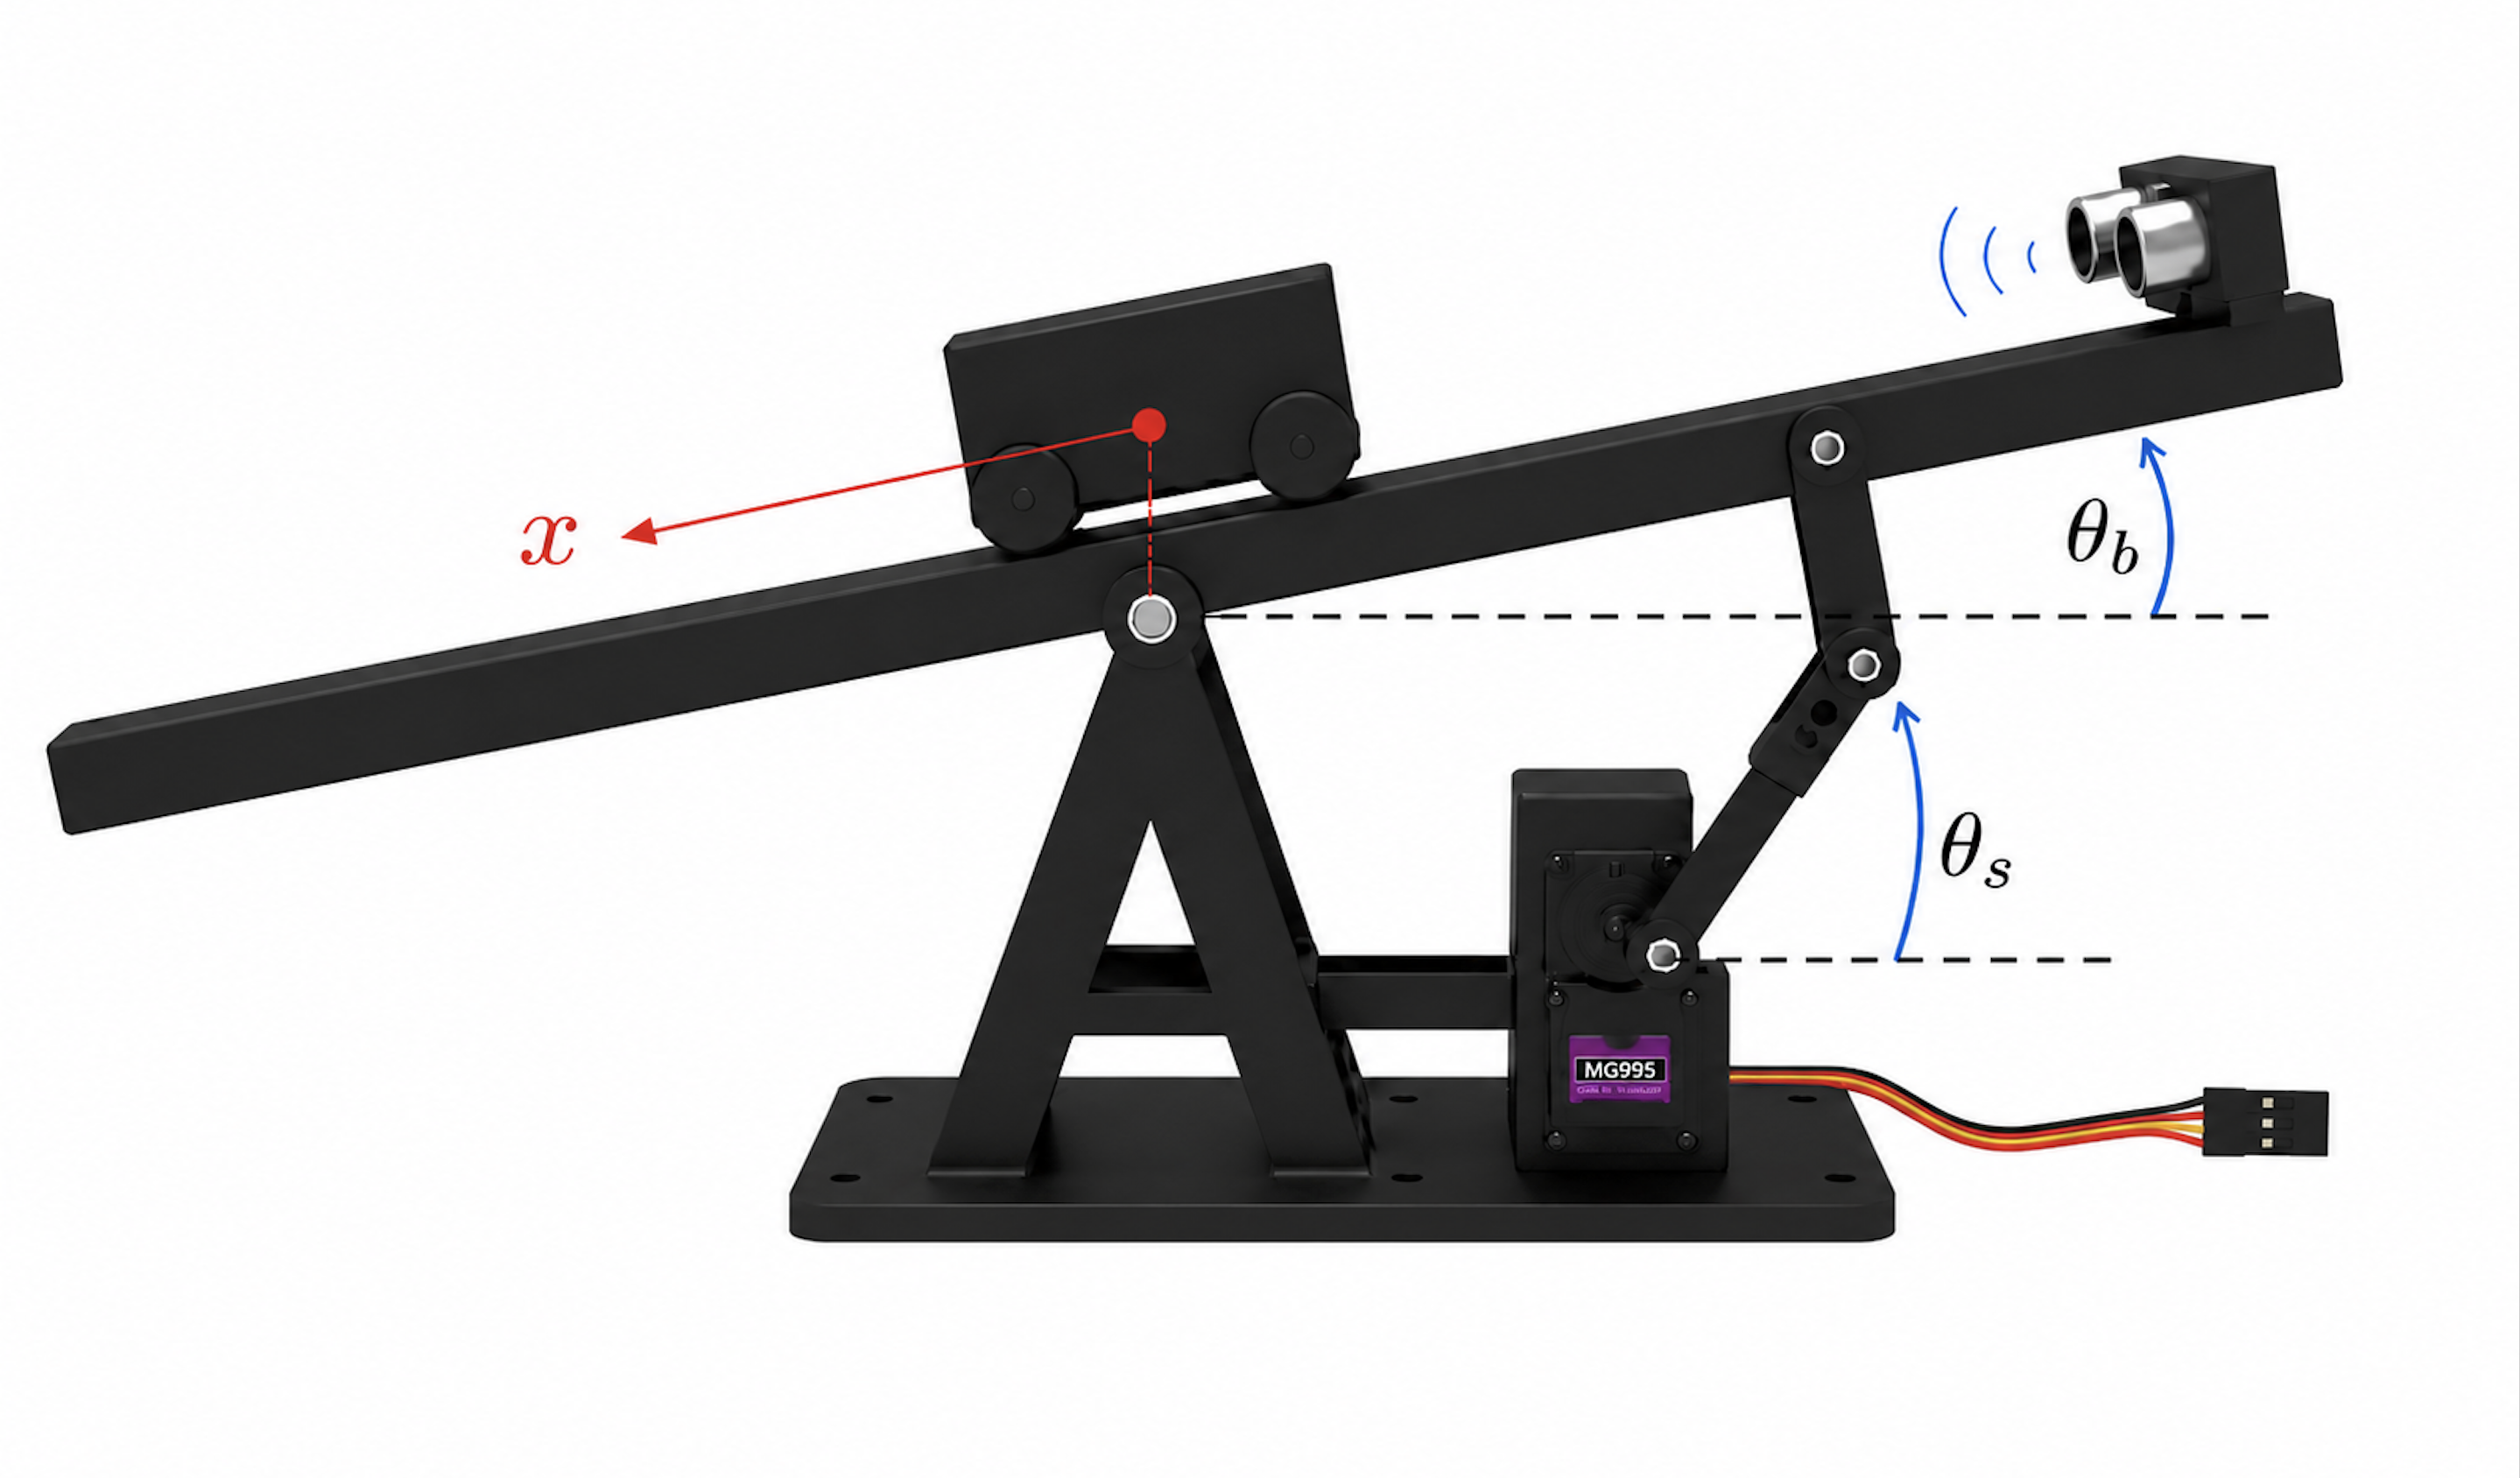
\includegraphics[width=0.8\textwidth]{img/planta.png}
    \caption{Sistema de referencia}
    \label{fig:sistema de referencia}
\end{figure}


Se tiene una barra de \SI{40}{\centi \meter} de longitud controlada por un servomotor sobre la cual se apoya un carrito. Mirando el servomotor de frente se considerna los $x$ positivos hacia la izquierda y los ángulos positivos en sentido antihorario. El origen de coordenadas para la posición es el centro de la barra y el ángulo $\theta_b = 0$ se produce para la barra horizontal. La \autoref{fig:sistema de referencia} ilustra el sistema de referencia adoptado.

Puede definirse un sistema en el que el ángulo comandado al servomotor $u$ es la entrada y la posición del carro es la salida. Se linealizó al mismo en torno al punto de equilibrio $(\theta_b, x) = (0, 0)$ y se halló su representación en espacio de estados.

\begin{minipage}{0.4\textwidth}
    \[
    \begin{cases}
    x_1 = \theta_b : \text{ángulo de la barra} \\
    x_2 = \dot{\theta}_b : \text{velocidad angular de la barra} \\
    x_3 = x : \text{posición del carro} \\
    x_4 = \dot{x} : \text{velocidad del carro}
    \end{cases}
    \]
\end{minipage}%
\begin{minipage}{0.4\textwidth}
\centering
    \begin{equation}
        x =
        \begin{bmatrix}
        x_1 \\
        x_2 \\
        x_3 \\
        x_4
        \end{bmatrix}
        \label{eq:vector de estados}
    \end{equation}
\end{minipage}

La \autoref{eq:vector de estados} muestra el vector de estados adoptado para este problema, en donde las dos primeras variables están asociadas al ángulo de la barra y las dos últimas a la posición del carro. Para este sistema de referencia y este vector de estados ya se había llegado a una representación del sistema en espacio de estados, la cual se repite aquí. 

\[
A=
\begin{bmatrix}
0 & 1 & 0 & 0 \\
-33,1549 & -9,7360 & 0 & 0 \\
0 & 0 & 0 & 1 \\
35,9445 & 0 & 0 & -10
\end{bmatrix}
\qquad
B=
\begin{bmatrix}
0 \\
11,4345 \\
0 \\
0
\end{bmatrix}
\]

\[
C=
\begin{bmatrix}
0 & 0 & 1 & 0
\end{bmatrix}
\qquad
D=
\begin{bmatrix}
0
\end{bmatrix}
\]

Cabe aclarar que este conjunto de matrices es válido si se consider que la salida del sistema es la posición del carro. Si además se quiere considerar el ángulo de la barra como salida, debe reemplazarse la matriz $C$ por: 

\[
C = \begin{bmatrix}
    0 & 0 & 1 & 0 \\
    1 & 0 & 0 & 0 
\end{bmatrix}
\]
.

Por último, de esta representación en espacio de estados puede obtenerse una función de transferencia.

\begin{equation}
\begin{aligned}
P(s) &= \frac{X(s)}{\Theta_s(s)}
      = \frac{k}{s(s-p_1)(s-p_2)(s-p_3)} \\
     &= \frac{410,7144}
{s\left(s+4,8680-3,0753j\right)\left(s+4,8680+3,0753j\right)(s+10)}
\end{aligned}
\end{equation}

\section{Diseño del observador}
A partir de la representación en espacio de estados descripta en la sección anterior se implementó un obsercador de Luenberger considerando la posición del carro y el ángulo de la barra como salidas del sistema. 

En primer lugar, debe verificarse la observabilidad del sistema, para lo cual es necesario que la matriz de observabilidad $\mathcal{O}$ sea de rango completo. Para un sistema de orden 4, dicha matriz se puede calcular como:

\begin{equation*}
    \mathcal{O} = 
    \begin{bmatrix}
        C \\
        CA \\ 
        CA^2 \\
        CA^3
    \end{bmatrix}.
\end{equation*}

En esta ecuación el valor de $C$ depende de qué variables de estado se consideren como salida del sistema (posición, ángulo de la barra o ambas). Analizando el rango de $\mathcal{O}$ para los distintos casos, se obtuvo que el sistema no es observable si solo se considera el ángulo de la barra como salida. Sin embargo, si se considera la posición o la posición y el ángulo de la barra como salidas, el mismo resulta observable.

Paralelamente, se analizó la controlabilidad del sistema a través del rango de la matriz de controlabilidad $\mathcal{C} = \begin{bmatrix}
    B & AB & A^2B & A^3B
\end{bmatrix}$. Se obtuvo que para todos los casos el sistema resulta controlable.

Una vez establecido que el sistema es observable se diseñó un observador de Luenberger a través de la técnica de \textit{pole placement} y la función \texttt{place} de \texttt{Matlab}.  

\begin{center}
\begin{minipage}{0.65\textwidth}
    \begin{subequations}
    \begin{align}
        \hat{x}_{k+1} &= A_d \hat{x}_k + L\left(y_k - \hat{y}_k\right) + B_d u_k 
        \label{eq:observador 1}
        \\
        \hat{y}_k &= C_d \hat{x}_k + D_d u_k
        \label{eq:observador 2}
    \end{align}
    \end{subequations}
\end{minipage}
\hfill
\begin{minipage}{0.30\textwidth}
\begin{equation}
e_{k+1} = \left(A_d - L C_d\right)e_k
\label{eq:error}
\end{equation}
\end{minipage}
\end{center}

Las ecuaciones \ref{eq:observador 1} y \ref{eq:observador 2} definen el observador, donde $\hat{x}_k$ es la estimación del vector de estados $x_k$ en el instante $k$. Se define además el error $e_k$ como $e_k = \hat{x}_k - x_k$, cuya evolución en el tiempo está dada por la \autoref{eq:error}. De esta forma, deben elegirse los valores de $L \in \mathbb{R}^{4 \times 2}$ tales que los autovalores de $A_d - LC_d$ sean más rápidos que las dinámicas de la planta. Sin embargo, los polos no deben ser demasiado rápidos para no añadir mucho ruido en la estimación, por lo cual se eligen autovalores entre 3 y 5 veces más rápidos que las dinámica asociadas a la planta, para luego ajustarlos en función de los gráficos obtenidos. 

Con estas consideraciones se eligieron los polos (en radianes por segundo)

\[
    \begin{bmatrix}
    -50 & -50 &-30 & -30
    \end{bmatrix}
\]

lo cual da por resultado la siguiente matriz $L$
\[
L=
\begin{bmatrix}
0      & 0.8886 \\
0      & 4.9459 \\
0.8833 & 0 \\
5.4272 & 0.7189
\end{bmatrix}
\]

Para corroborar el buen funciomaniento del observador se realizaron gráficos superponiendo las variables de estado medidas, observadas y simuladas. Como entrada se aplicó un tren de escalones de $\pm \SI{20}{\degree}$ con un período de $\SI{1,2}{\s}$.

\begin{figure}[H]
    \centering
    
\includegraphics[width=0.9\textwidth]{img/obs_img/pos.pdf}
    \caption{Posición del carro}
    \label{fig:pos_obs}
\end{figure}

\begin{figure}[H]
    \centering
    
\includegraphics[width=0.9\textwidth]{img/obs_img/vel.pdf}
    \caption{Velocidad del carro}
    \label{fig:vel_obs}
\end{figure}

No se grafica la estimación de la velocidad a partir de los datos del sensor ya que resultó excesivamente ruidosa y entorpecía la imagen. 

\begin{figure}[H]
    \centering
    
\includegraphics[width=0.9\textwidth]{img/obs_img/ang.pdf}
    \caption{Ángulo de la barra}
    \label{fig:ang_obs}
\end{figure}

\begin{figure}[H]
    \centering
    
\includegraphics[width=0.9\textwidth]{img/obs_img/velang.pdf}
    \caption{Velocidad angular de la barra}
    \label{fig:velang_obs}
\end{figure}

Se observa que en general la estimación de las variables de estado es similar a la medición y a la simulación. Esto no se cumple para la posición (figura \ref{fig:pos_obs}), lo que se atribuye a las asimetrías y alinealidades de la planta. 

\section{Controlador por realimentación de estados}

En la presente sección se desarrolla el diseño de controladores por realimentación de variables de estado.

El primer diseño consiste en estabilizar al sistema en torno al punto de equilibrio $ E = \left( p_e = 0\,\text{cm}, ~ \theta_e = 0\text{°} \right)$ naturalmente, sin seguimiento de referencias.

El segundo diseño añade la matriz de \textit{feed-forward} para el seguimiento de referencias $
r_k =
\begin{bmatrix}
p_\text{ref} & \theta_\text{ref}
\end{bmatrix}^\text{T}
$.

El tercer y último diseño involucra acción integral.

\subsection{Estabilización al punto de equilibrio}
\subsubsection{Diseño teórico}

El desarrollo del observador de Luenberger permite obtener mejores estimaciones de las variables de estado a un nivel de bajo ruido en comparación con los valores arrojados por los sensores. De este modo, la ley de control se implementa sobre el vector de estados estimados $\widehat{x_k}$ y se reescribe el modelo discreto de la representación en variables de estado como
\begin{align*}
\widehat{x_{k+1}} &= A_d \, \widehat{x_k} + B_d \, u_k\,, \\
y_k &= C_d \, \widehat{x_k} + D_d \, u_k \, , \\
u_k &= K \, \widehat{x_k} \, ,
\end{align*}
donde
\[
\widehat{x}_k,\ \widehat{x}_{k+1} \in \mathbb{R}^4,\qquad
u_k \in \mathbb{R},\qquad
y_k \in \mathbb{R}^2,
\]
\[
A_d \in \mathbb{R}^{4\times4},\qquad
B_d \in \mathbb{R}^{4\times1},\qquad
C_d \in \mathbb{R}^{2\times4},\qquad
D_d \in \mathbb{R}^{2\times1},
\]
\[
K \in \mathbb{R}^{1\times4}.
\]

Por tanto, se obtiene la relación
\[
\widehat{x_{k+1}} = \left( A_d + B_d \, K \right) \widehat{x_k}
\]
de donde el sistema es estable si los autovalores de $\left( A_d + B_d \, K \right)$ se encuentran dentro del círculo unitario. Esos autovalores representan los polos discretos del sistema a lazo cerrado, por lo que escogiéndolos oportunamente se determinará una matriz $K$ específica para la realimentación.

Para la elección de los polos del controlador se buscó separar la dinámica rápida de la dinámica lenta del sistema, de manera de poder interpretar la respuesta en lazo cerrado en términos de polos dominantes. Con ese criterio, se definió un polo real doble,
\[
p_1 = p_2 = -10\,,
\]
ubicado considerablemente más a la izquierda que el segundo par de polos. Al tratarse de un polo rápido y bien amortiguado, su contribución a la respuesta transitoria decae en una fracción muy pequeña del tiempo de establecimiento total, por lo que su efecto resulta prácticamente despreciable frente al del resto de la dinámica. De este modo, $p_1$ y $p_2$ no imponen restricciones sobre la velocidad ni la forma de la respuesta global, sino que únicamente garantizan una rápida extinción de los modos asociados a ellos, dejando que la dinámica dominante quede determinada por el segundo par de polos.

Dicho segundo par se planteó en forma compleja conjugada,
\[
p_3 = 5\,e^{\,j\,100\text{°}}\,, \qquad p_4 = \overline{p_3}\,,
\]
con factor de amortiguamiento $\zeta \approx 0,174$. Esta elección, en lugar de polos puramente reales, responde a la naturaleza misma de la planta \textit{ball and beam}: al tratarse de un sistema con dos grados de libertad acoplados —la posición del carrito sobre la barra y el ángulo de inclinación—, su dinámica natural es oscilatoria, con intercambio de energía entre ambas variables. Forzar un comportamiento críticamente amortiguado (polos reales) resulta poco representativo de esta física y, además, demanda una acción de control excesivamente agresiva. El par complejo conjugado permite capturar este acoplamiento natural y, al ser dominante por sobre $p_1$ y $p_2$, determina el sobrepico y el tiempo de establecimiento del sistema, evitando al mismo tiempo que la acción de control $u_k$ sature los límites mecánicos del servo.

Cabe destacar que estos polos del controlador deben ser, además, más lentos que los del observador, de modo que la estimación de los estados converja antes de que la ley de control actúe sobre ella; de no cumplirse esta relación, la realimentación operaría sobre estimaciones poco confiables, degradando el desempeño del lazo cerrado.

Finalmente, los polos en su forma continua y su equivalente discreto (obtenido mediante $z = e^{s\,T_S}$, con $T_S = 0,02\,\text{s}$) quedan expresados como
\[
\begin{aligned}
p_1 &= p_2 = -10 \,, & z_1 &= z_2 = 0,8187\,, \\[4pt]
p_3 &= -0,8682 + 4,9240\,j\,, & z_3 &= 0,9780 + 0,0967\,j\,, \\[4pt]
p_4 &= -0,8682 - 4,9240\,j\,, & z_4 &= 0,9780 - 0,0967\,j\,.
\end{aligned}
\]

A partir de estos cuatro polos se calculó la matriz de realimentación mediante la función \texttt{place} de MATLAB, obteniéndose
\[
K = \begin{bmatrix} -0,8952 & -0,0586 & -4,9511 & -0,4751 \end{bmatrix}\,.
\]

\subsubsection{Verificación experimental}

Para verificar el diseño del controlador, se sometió el sistema a condiciones iniciales no nulas y se compararon las variables de estado observadas con las simuladas, tal y como muestra la Figura~\ref{fig:realim-estados}. 

En la Figura~\ref{fig:realim-pos} se muestra que la posición del carrito observada tiene menor sobrepico que la simulada y posee un error no
nulo en estado estacionario debido al rozamiento estático propio de la planta.

En la Figura~\ref{fig:realim-velang} se muestra que la velocidad angular observada tiene menor sobrepico que la simulada y se establece correctamente sin error en estado estacionario.

La Figura~\ref{fig:realim-ang} muestra que el ángulo de la barra observado es similar al simulado, con algo menos de sobrepico en el caso observado y con un error no nulo en estado estacionario debido a que el controlador intenta corregir el error en estado estacionario de la posición del carrito poniendo una acción de control constante pero insuficiente, debido al rozamiento. Esto hace que el observador persiba una velocidad del carrito constante no nula en estado estacionario, tal y como se muestra en la Figura~\ref{fig:realim-vel}.

Asimismo, la Figura~\ref{fig:realim-uk} muestra la acción de control comandada, en acuerdo con lo dicho en el párrafo anterior.

\begin{figure}[H]
    \centering
    \begin{subfigure}{0.48\textwidth}
        \centering
        
\includegraphics[width=\linewidth]{img/realim_img/pos.pdf}
        \caption{Posición del carrito.}
        \label{fig:realim-pos}
    \end{subfigure}
    \hfill
    \begin{subfigure}{0.48\textwidth}
        \centering
        
\includegraphics[width=\linewidth]{img/realim_img/vel.pdf}
        \caption{Velocidad del carrito.}
        \label{fig:realim-vel}
    \end{subfigure}

    \vspace{0.3cm}

    \begin{subfigure}{0.48\textwidth}
        \centering
        
\includegraphics[width=\linewidth]{img/realim_img/ang.pdf}
        \caption{Ángulo de la barra.}
        \label{fig:realim-ang}
    \end{subfigure}
    \hfill
    \begin{subfigure}{0.48\textwidth}
        \centering
        
\includegraphics[width=\linewidth]{img/realim_img/velang.pdf}
        \caption{Velocidad angular de la barra.}
        \label{fig:realim-velang}
    \end{subfigure}
    \caption{Variables de estado del sistema con realimentación de estados a condiciones iniciales no nulas observadas y simuladas.}
    \label{fig:realim-estados}
\end{figure}

\begin{figure}[H]
    \centering
    
\includegraphics[width=0.7\textwidth]{img/realim_img/uk.pdf}
    \caption{Acción de control comanda al sistema ante condiciones iniciales no nulas.}
    \label{fig:realim-uk}
\end{figure}

\subsection{Seguimiento de referencias}
\subsubsection{Diseño teórico}

Con el objetivo de habilitar el seguimiento de referencias en el sistema a lazo cerrado, se incorpora un término adicional a la ley de control, ponderado por una matriz de \textit{feed-forward} $F$, que actúa directamente sobre la referencia y se combina con la realimentación de estados. La acción de control resulta entonces
\[
u_k = K\,\widehat{x_k} + F\,r_k\,,
\]
con
\[
F \in \mathbb{R}^{1\times 2}\,, \qquad r_k \in \mathbb{R}^{2}\,.
\]
Sustituyendo esta expresión en el modelo discreto del sistema, se obtiene
\[
\widehat{x_{k+1}} = (A_d + B_d K)\,\widehat{x_k} + B_d\,F\,r_k\,,
\]
a partir de lo cual puede despejarse la condición que debe cumplir $F$ para que la salida converja a la referencia en régimen estacionario:
\[
F = \left( C_d\,(\mathbf{I} - (A_d + B_d K))^{-1} B_d \right)^{-1}\,.
\]
Dado que se busca seguir simultáneamente una referencia de posición $p$ y una de ángulo $\theta$, y empleando la matriz $K$ obtenida en el diseño previo, el cálculo arroja
\[
F = \begin{bmatrix} 4,9511 & 0 \end{bmatrix}\,.
\]
Cabe aclarar que esta ``inversa'' no es tal en sentido estricto sino una pseudoinversa, ya que el producto $C_d (\mathbf{I}-(A_d + B_d K))^{-1} B_d$ da como resultado un vector columna de $2\times 1$ y no una matriz cuadrada. Esto trae como consecuencia que el controlador no pueda imponer ambas referencias de forma independiente. La componente correspondiente a la referencia angular resulta nula, lo cual tiene sentido físico: en estado estacionario, el carrito solo puede permanecer quieto en una posición fija si la barra está horizontal ($\theta = 0$), por lo que no es posible sostener una referencia de ángulo distinta de cero sin que el carrito continúe desplazándose indefinidamente.

\subsubsection{Verificación experimental}

Se comandó un tren de escalones asimétricos entre $-8\,$cm y $2\,$cm como referencia para la posición del carrito y una referencia nula para el ángulo de la barra. Las variables de estado observadas y simuladas se muestran en la Figura~\ref{fig:ref-estados}.

En la Figura~\ref{fig:ref-pos} se observa que la posición del carrito sigue la forma general de la referencia, aunque con sobrepicos importantes ante cada cambio de escalón. Además, la respuesta observada presenta un error no nulo en estado estacionario, asociado nuevamente al rozamiento estático de la planta y a la ausencia de acción integral en este diseño.

La Figura~\ref{fig:ref-vel} muestra que la velocidad observada presenta picos pronunciados durante los transitorios, en especial al inicio de cada cambio de referencia. Luego, tiende a valores aproximadamente constantes o cercanos a cero según el tramo, lo cual es consistente con el error estacionario observado en la posición.

En la Figura~\ref{fig:ref-ang} se aprecia que el ángulo de la barra actúa como variable intermedia para desplazar el carrito hacia la nueva referencia. En régimen estacionario, el ángulo observado no siempre converge exactamente a cero, debido a que el controlador debe sostener una inclinación residual para compensar parcialmente los efectos de fricción.

Finalmente, la Figura~\ref{fig:ref-velang} muestra que la velocidad angular concentra su mayor actividad durante los cambios de escalón. La respuesta observada resulta más abrupta que la simulada, lo que evidencia las limitaciones del modelo ideal frente a la dinámica real del actuador, el rozamiento y el ruido de medición.

Asimismo, la Figura~\ref{fig:ref-uk} muestra la acción de control comandada para el seguimiento de referencias, en la cual se observan variaciones abruptas ante cada cambio de escalón y valores sostenidos durante los intervalos en los que el controlador compensa el error estacionario de posición.

\begin{figure}[H]
    \centering
    \begin{subfigure}{0.48\textwidth}
        \centering
        
\includegraphics[width=\linewidth]{img/ref_img/pos.pdf}
        \caption{Posición del carrito.}
        \label{fig:ref-pos}
    \end{subfigure}
    \hfill
    \begin{subfigure}{0.48\textwidth}
        \centering
        
\includegraphics[width=\linewidth]{img/ref_img/vel.pdf}
        \caption{Velocidad del carrito.}
        \label{fig:ref-vel}
    \end{subfigure}

    \vspace{0.3cm}

    \begin{subfigure}{0.48\textwidth}
        \centering
        
\includegraphics[width=\linewidth]{img/ref_img/ang.pdf}
        \caption{Ángulo de la barra.}
        \label{fig:ref-ang}
    \end{subfigure}
    \hfill
    \begin{subfigure}{0.48\textwidth}
        \centering
        
\includegraphics[width=\linewidth]{img/ref_img/velang.pdf}
        \caption{Velocidad angular de la barra.}
        \label{fig:ref-velang}
    \end{subfigure}
    \caption{Variables de estado del sistema con realimentación de estados y seguimiento de referencias observadas y simuladas.}
    \label{fig:ref-estados}
\end{figure}

\begin{figure}[H]
    \centering
    
\includegraphics[width=0.7\textwidth]{img/ref_img/uk.pdf}
    \caption{Acción de control comandada al sistema durante el seguimiento de referencias.}
    \label{fig:ref-uk}
\end{figure}

\subsection{Acción integral}

\subsection{Rediseño del observador}

A la hora de diseñar el control con acción integral, se encontró que el observador introducía demasiado ruido en la acción de control. Por esto se decidió modificar los valores de los polos elegidos para mitigar este efecto. Los nuevos valores en el dominio continuo fueron

\[
    \begin{bmatrix}
    -25 & -25 & -10 & -10
    \end{bmatrix}\, .
\] 

De esta forma, se consiguió una acción de control más estable. Si bien estos polos son comparables con la dinámica más rápida de la planta, en la práctica el observador funcionó de forma eficiente. Esto puede atribuirse a una identificación incorrecta de la planta, y a que el polo más rápdo de la misma sea en realidad menor. 

\subsubsection{Diseño teórico}

Con el fin de eliminar el error en estado estacionario producido por la fricción —inevitable en el sistema físico—, se incorpora una acción integral al esquema de control. El objetivo de diseño en esta etapa, además de garantizar error nulo en régimen permanente, es lograr una respuesta rápida: tiempo de establecimiento inferior a $2,5\,\text{s}$ y sobrepico inferior al $15\%$.

Para ello se define una nueva variable de estado $q$, correspondiente a la integral del error entre la referencia $r$ y la salida medida:
\[
\dot{q} = r - C\,x\,.
\]
La acción de control queda entonces compuesta tanto por la realimentación de los estados originales como por este nuevo estado integrador:
\[
u = H\,q + K\,x = \begin{bmatrix} K & H \end{bmatrix} \begin{bmatrix} x \\ q \end{bmatrix}\,.
\]

Incorporando la dinámica del integrador, se obtiene el sistema aumentado
\[
\begin{bmatrix} \dot{x} \\ \dot{q} \end{bmatrix}
=
\begin{bmatrix} A & 0 \\ -C & 0 \end{bmatrix}
\begin{bmatrix} x \\ q \end{bmatrix}
+
\begin{bmatrix} B \\ 0 \end{bmatrix} u
+
\begin{bmatrix} 0 \\ 1 \end{bmatrix} r\,,
\]
y reemplazando la ley de control $u = \begin{bmatrix} K & H \end{bmatrix}\begin{bmatrix} x \\ q \end{bmatrix}$, queda
\[
\begin{bmatrix} \dot{x} \\ \dot{q} \end{bmatrix}
=
\left(
\begin{bmatrix} A & 0 \\ -C & 0 \end{bmatrix}
+
\begin{bmatrix} B \\ 0 \end{bmatrix}
\begin{bmatrix} K & H \end{bmatrix}
\right)
\begin{bmatrix} x \\ q \end{bmatrix}
+
\begin{bmatrix} 0 \\ 1 \end{bmatrix} r\,.
\]

Llevando esta formulación a tiempo discreto, con el observador de Luenberger ya incorporado, el sistema aumentado resulta
\[
\begin{bmatrix} \widehat{x_{k+1}} \\ q_{k+1} \end{bmatrix}
=
\left(
\underbrace{\begin{bmatrix} A_d & 0 \\ -C_d\,T_s & 1 \end{bmatrix}}_{\widehat{A}_d}
+
\underbrace{\begin{bmatrix} B_d \\ 0 \end{bmatrix}}_{\widehat{B}_d}
\underbrace{\begin{bmatrix} K & H \end{bmatrix}}_{\widehat{K}}
\right)
\begin{bmatrix} \widehat{x_k} \\ q_k \end{bmatrix}
+
\begin{bmatrix} 0 \\ 1 \end{bmatrix} r_k\,,
\]
donde el estado integrador se actualiza, de forma discreta, mediante
\[
q_k = q_{k-1} + T_s\,(r_k - y_k)\,.
\]
Al igual que en el diseño anterior, la elección de los autovalores de $\left( \widehat{A}_d + \widehat{B}_d\,\widehat{K} \right)$ —ahora dentro del círculo unitario, en un espacio de estados de dimensión $5$— determina la matriz de ganancias aumentada $\widehat{K} = \begin{bmatrix} K & H \end{bmatrix}$, calculada nuevamente mediante \texttt{place}.

A diferencia del diseño anterior, donde se buscaba estabilizar simultáneamente el ángulo y la posición, en este caso solo se desea controlar la posición $p$ del carrito (el ángulo continúa siendo medido para el observador, pero no se generan referencias para la barra), por lo que $C_d = \begin{bmatrix} 0 & 0 & 1 & 0 \end{bmatrix}$. 

Los polos seleccionados fueron
\[
p_1 = -7,00\,; \quad p_2 = -2,80 \,; \quad p_3 = -8,10 \,; \quad p_4 = -2,81 \,; \quad p_5 = -6,00 \,.    
\]

Discretizando los polos continuos mediante $z = e^{s\,T_s}$, se obtienen los polos discretos
\[
z_1 = 0,8694\,; \qquad z_2 = 0,9455\,; \qquad z_3 = 0,8504\,; \quad z_4 = 0,9454\,; \quad z_5 = 0,8869 \, .
\]

Aplicando \texttt{place} sobre el par $(\widehat{A}_d, \widehat{B}_d)$ con estos polos discretos, se obtuvo la matriz de ganancias aumentada, separada en su componente sobre los estados originales $K$ y su componente sobre el estado integrador $H$:
\[
K = \begin{bmatrix} -5,1097 & -0,4708 & -5,9842 & -0,4995 \end{bmatrix}\,, \qquad H = 4,9998\,.
\]
Mientras que $K$ pondera los cuatro estados originales del sistema (ángulo, velocidad angular, posición y velocidad), $H$ pondera al estado integrador $q$, es decir, actúa como la ganancia proporcional al error acumulado de posición, siendo la responsable directa de eliminar el error en estado estacionario.

\subsubsection{Verificación experimental}

Se comandó un tren de escalones simétricos entre $-8\,$cm y $8\,$cm como referencia para la posición del carrito. Las variables de estado observadas y simuladas se muestran en la Figura~\ref{fig:ai-estados}, mientras que la acción de control aplicada se presenta en la Figura~\ref{fig:ai-uk}.

En la Figura~\ref{fig:ai-pos} se observa que, a diferencia del caso sin acción integral, la posición del carrito reduce considerablemente el error en estado estacionario, aunque este no llega a ser estrictamente nulo. Para el cambio de referencia de $8\,$cm a $-8\,$cm, y despreciando el ruido de medición, el mínimo observado es cercano a $-9,3\,$cm. Dado que la amplitud del escalón es de $16\,$cm, esto equivale a un sobrepico real de aproximadamente $8\,$\%, menor que el límite de diseño del $15\,$\%. Asimismo, el tiempo de establecimiento se estima en aproximadamente $2,2\,$s, también menor que la especificación de $2,5\,$s. La acción integral es la responsable de esta reducción del error estacionario: mientras existe diferencia entre la referencia y la posición medida, la integral del error se acumula y modifica la acción de control hasta compensar parcialmente los efectos de rozamiento de la planta.

La Figura~\ref{fig:ai-vel} muestra que la velocidad del carrito presenta picos durante los cambios de referencia y luego tiende a reducirse a medida que la posición se establece. Durante el tramo de referencia positiva aparecen oscilaciones superpuestas, asociadas a la vibración mecánica de la barra y no a un cambio sostenido de referencia.

En la Figura~\ref{fig:ai-ang} se aprecia que el ángulo de la barra acompaña los cambios de referencia y presenta oscilaciones más notorias cuando el carrito sigue referencias positivas, correspondientes a la mitad izquierda de la barra según la Figura~\ref{fig:sistema de referencia}. En esa zona, el peso del carrito ejerce un torque sobre la barra que tiende a hacerla caer levemente; sin embargo, la causa principal de las vibraciones observadas es que la acción de control resulta muy ruidosa debido al ruido intrínseco del sensor ultrasónico. Esto ocurre aun habiendo corregido el observador y exigiéndolo casi al máximo, de modo que el servo recibe una señal con variaciones rápidas y las reproduce como oscilaciones mecánicas en la barra.

La Figura~\ref{fig:ai-velang} confirma este comportamiento: la velocidad angular exhibe oscilaciones durante los tramos en los que la barra vibra y picos importantes ante cada cambio de escalón. Estas oscilaciones no aparecen con la misma intensidad en la simulación, ya que el modelo no reproduce completamente la flexibilidad, los juegos mecánicos ni las perturbaciones asociadas al montaje real.

Finalmente, la Figura~\ref{fig:ai-uk} muestra que la acción de control presenta una componente oscilatoria importante mientras el carrito se encuentra en la zona de referencia positiva, justamente donde la vibración de la barra es más notoria. Luego del cambio hacia la referencia negativa, la señal de control realiza una corrección intensa para invertir el movimiento y, posteriormente, converge hacia el valor necesario para sostener el carrito en la nueva posición. Esta evolución es coherente con la acción integral: ante error acumulado, el controlador incrementa o reduce la señal de mando hasta cancelar el error de posición, aunque las vibraciones y el ruido introducen oscilaciones adicionales sobre dicha señal.

\begin{figure}[H]
    \centering
    \begin{subfigure}{0.48\textwidth}
        \centering
        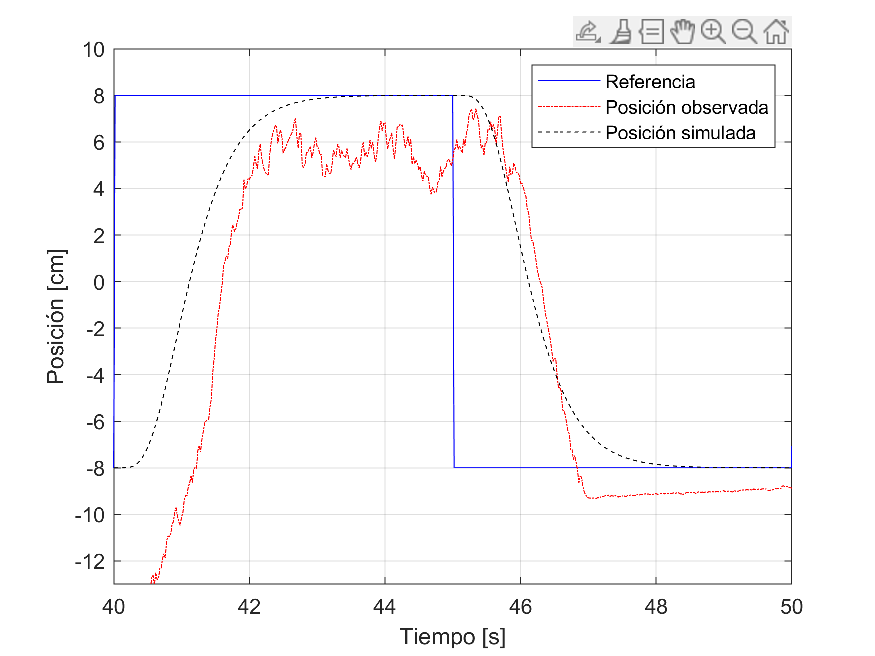
\includegraphics[width=\linewidth]{img/AI_img/pos.pdf}
        \caption{Posición del carrito.}
        \label{fig:ai-pos}
    \end{subfigure}
    \hfill
    \begin{subfigure}{0.48\textwidth}
        \centering
        
\includegraphics[width=\linewidth]{img/AI_img/vel.pdf}
        \caption{Velocidad del carrito.}
        \label{fig:ai-vel}
    \end{subfigure}

    \vspace{0.3cm}

    \begin{subfigure}{0.48\textwidth}
        \centering
        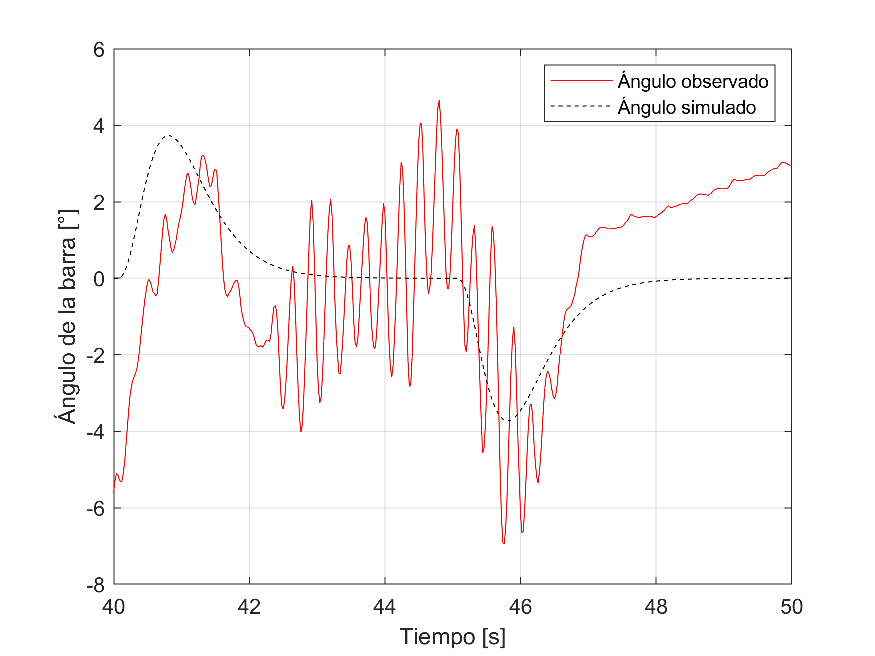
\includegraphics[width=\linewidth]{img/AI_img/ang.pdf}
        \caption{Ángulo de la barra.}
        \label{fig:ai-ang}
    \end{subfigure}
    \hfill
    \begin{subfigure}{0.48\textwidth}
        \centering
        
\includegraphics[width=\linewidth]{img/AI_img/velang.pdf}
        \caption{Velocidad angular de la barra.}
        \label{fig:ai-velang}
    \end{subfigure}
    \caption{Variables de estado del sistema con acción integral durante el seguimiento de referencias observadas y simuladas.}
    \label{fig:ai-estados}
\end{figure}

\begin{figure}[H]
    \centering
    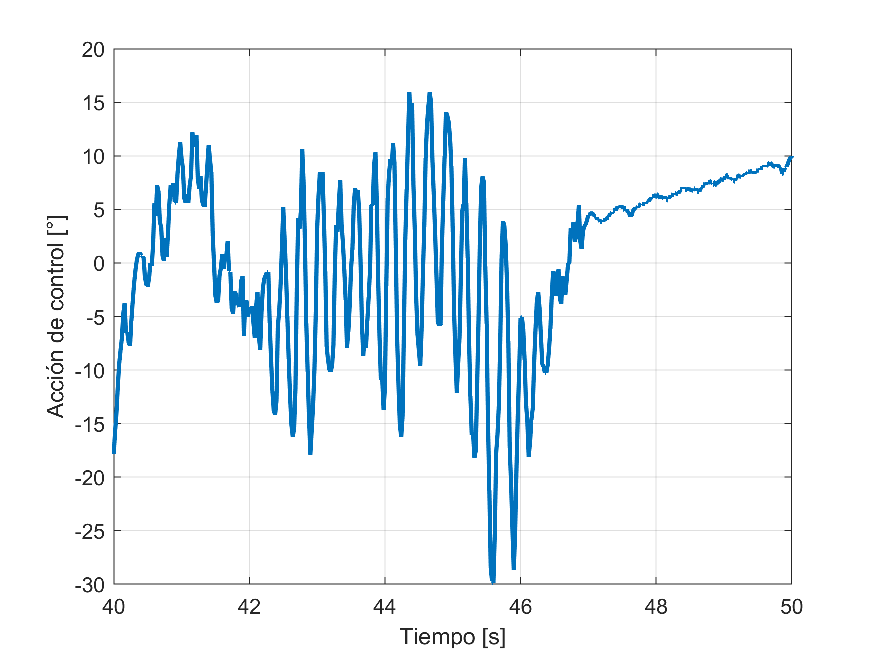
\includegraphics[width=0.7\textwidth]{img/AI_img/uk.pdf}
    \caption{Acción de control comandada al sistema con acción integral durante el seguimiento de referencias.}
    \label{fig:ai-uk}
\end{figure}


\section{Conclusiones}

En el desarrollo del trabajo se logró modelar la planta, verificar sus propiedades de observabilidad y controlabilidad, y diseñar un observador capaz de estimar las variables de estado necesarias para implementar las leyes de control. La comparación entre simulación y ensayo experimental mostró que el modelo captura adecuadamente la dinámica general del sistema, aunque no reproduce por completo efectos no ideales como rozamiento, juegos mecánicos, vibraciones estructurales y ruido de medición.

El controlador por realimentación de estados permitió estabilizar el sistema alrededor del punto de equilibrio, pero presentó error en estado estacionario en la posición del carrito debido principalmente al rozamiento estático. Al incorporar la matriz de \textit{feed-forward}, se consiguió seguir referencias de posición, aunque se verificó que no es posible imponer simultáneamente una referencia arbitraria de ángulo en régimen permanente, ya que físicamente el carrito solo puede permanecer quieto en una posición fija si la barra se mantiene horizontal.

La incorporación de acción integral redujo considerablemente el error estacionario y permitió cumplir, en la respuesta de posición, con un sobrepico menor al $15\,\text{\%}$ y un tiempo de establecimiento inferior a $2,5\,\text{s}$ para el ensayo considerado. Sin embargo, el error no se anuló completamente y aparecieron vibraciones asociadas a una acción de control ruidosa, principalmente por el ruido intrínseco del sensor ultrasónico aun con el observador corregido y exigido casi al máximo. Esto evidencia el compromiso entre rapidez de respuesta, rechazo de error estacionario, ruido de medición y esfuerzo de control.

En síntesis, los controladores diseñados permitieron validar experimentalmente las herramientas de realimentación de estados, observación y acción integral, y mostraron la importancia de considerar las limitaciones físicas de la planta al pasar del diseño teórico a la implementación real.



\end{document}